\section{Oppgave 1 - GPIO}\label{sec:3-oppgave-GPIO}


\subsection{Beskrivelse}



I denne oppgaven skal vi skru på alle LED-ene i matrisen når knappen \verb|B| trykkes, og skru dem av når knappen \verb|A| trykkes. Dette gjøres med \verb|GPIO|-modulene. Dette er moduler som har ansvarer for generell input og output (\verb|GPIO| = \textbf{G}eneral \textbf{P}urpose \textbf{I}nput \textbf{O}utput).

Denne oppgaven er strukturert som en walkthrough, for å introdusere konsepter som skal brukes i senere oppgaver. Tanken er at det blir gradvis mindre håndholding. Før dere starter er det lurt å skumlese appendiks \ref{app:datablad} og \ref{app:bit}.

I denne oppgaven, så trenger dere bare å endre på \verb|main.c|. De spesielt interesserte kan se på mappen \verb|.build_system| og \verb|Makefile|. Sistenevnte kan endres på om dere velger å lage flere \verb|.h| eller \verb|.c|-filer for at det skal bli ryddigere.

\begin{center}
 \begin{tabular}{|p{8.5cm} p{5.5cm}|} 
 \hline
 Filer & Skal denne filen endres?  \\ [0.5ex] 
 \hline\hline
 \verb|1_gpio/main.c| & \quad \quad \quad \quad ja  \\ 
 \hline
  \verb|1_gpio/.build_system| &  \quad \quad \quad \quad helst ikke \\ 
 \hline
 \verb|1_gpio/Makefile| &  \quad \quad \quad \quad helst ikke \\ 
 \hline
\end{tabular}
\end{center}


\subsection{Oppgave}

LED-matrisen på micro:bit-en består av en 5x5 matrise som har blitt implementert som en 5x5 matrise (se figur \ref{fig:microbit-led}). I denne matrisen er det egentlig ikke et system (i tidligere micro:bit så har rad 1-5 alltid vært etter hverandre med hensyn på pins. Det same gjaldt også kolonnene), hvor pinne 28, 11, 31, 5, og 30 tilsvarer jord, mens pinne 21, 22, 15, 24, og 19 tilsvarer  strømforsyning. Dermed, for å få diode nummer 12 til å lyse, må \verb|P31| være trukket lav, mens \verb|P15| være høy.

\begin{figure}[ht]
    \centering
    

\tikzset{every picture/.style={line width=0.75pt}} %set default line width to 0.75pt        

\resizebox{.6\textwidth}{!}{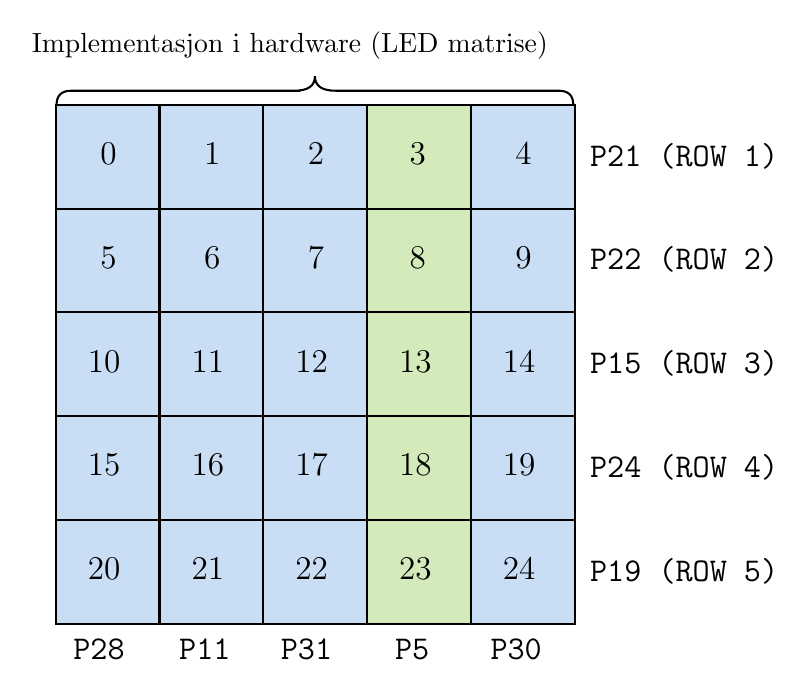
\begin{tikzpicture}[x=0.75pt,y=0.75pt,yscale=-1,xscale=1]
%uncomment if require: \path (0,650); %set diagram left start at 0, and has height of 650

%Shape: Brace [id:dp07590887393055623] 
\draw   (419.4,378.28) .. controls (419.4,373.61) and (417.07,371.28) .. (412.4,371.28) -- (304.9,371.28) .. controls (298.23,371.28) and (294.9,368.95) .. (294.9,364.28) .. controls (294.9,368.95) and (291.57,371.28) .. (284.9,371.28)(287.9,371.28) -- (177.4,371.28) .. controls (172.73,371.28) and (170.4,373.61) .. (170.4,378.28) ;
%Shape: Square [id:dp3773221579232766] 
\draw  [fill={rgb, 255:red, 201; green, 222; blue, 245 }  ,fill opacity=1 ] (170,378.08) -- (220,378.08) -- (220,428.08) -- (170,428.08) -- cycle ;
%Shape: Square [id:dp6702270611189987] 
\draw  [fill={rgb, 255:red, 201; green, 222; blue, 245 }  ,fill opacity=1 ] (220,378.08) -- (270,378.08) -- (270,428.08) -- (220,428.08) -- cycle ;
%Shape: Square [id:dp9219716969130087] 
\draw  [fill={rgb, 255:red, 201; green, 222; blue, 245 }  ,fill opacity=1 ] (270,378.08) -- (320,378.08) -- (320,428.08) -- (270,428.08) -- cycle ;
%Shape: Square [id:dp8001210146008937] 
\draw  [fill={rgb, 255:red, 201; green, 222; blue, 245 }  ,fill opacity=1 ] (170,428.08) -- (220,428.08) -- (220,478.08) -- (170,478.08) -- cycle ;
%Shape: Square [id:dp25979952621996283] 
\draw  [fill={rgb, 255:red, 201; green, 222; blue, 245 }  ,fill opacity=1 ] (170,478.08) -- (220,478.08) -- (220,528.08) -- (170,528.08) -- cycle ;
%Shape: Square [id:dp9196426147745322] 
\draw  [fill={rgb, 255:red, 201; green, 222; blue, 245 }  ,fill opacity=1 ] (170,528.08) -- (220,528.08) -- (220,578.08) -- (170,578.08) -- cycle ;
%Shape: Square [id:dp41457626400817027] 
\draw  [fill={rgb, 255:red, 201; green, 222; blue, 245 }  ,fill opacity=1 ] (170,578.08) -- (220,578.08) -- (220,628.08) -- (170,628.08) -- cycle ;
%Shape: Square [id:dp3582088774997647] 
\draw  [fill={rgb, 255:red, 201; green, 222; blue, 245 }  ,fill opacity=1 ] (220,578.08) -- (270,578.08) -- (270,628.08) -- (220,628.08) -- cycle ;
%Shape: Square [id:dp3109259000247424] 
\draw  [fill={rgb, 255:red, 201; green, 222; blue, 245 }  ,fill opacity=1 ] (270,578.08) -- (320,578.08) -- (320,628.08) -- (270,628.08) -- cycle ;
%Shape: Square [id:dp015124928185211495] 
\draw  [fill={rgb, 255:red, 211; green, 235; blue, 187 }  ,fill opacity=1 ] (320,578.08) -- (370,578.08) -- (370,628.08) -- (320,628.08) -- cycle ;
%Shape: Square [id:dp2025768158998178] 
\draw  [fill={rgb, 255:red, 201; green, 222; blue, 245 }  ,fill opacity=1 ] (370,578.08) -- (420,578.08) -- (420,628.08) -- (370,628.08) -- cycle ;
%Shape: Square [id:dp4409776036060886] 
\draw  [fill={rgb, 255:red, 211; green, 235; blue, 187 }  ,fill opacity=1 ] (320,378.08) -- (370,378.08) -- (370,428.08) -- (320,428.08) -- cycle ;
%Shape: Square [id:dp7188431002318938] 
\draw  [fill={rgb, 255:red, 201; green, 222; blue, 245 }  ,fill opacity=1 ] (370,378.08) -- (420,378.08) -- (420,428.08) -- (370,428.08) -- cycle ;
%Shape: Square [id:dp5255474217407516] 
\draw  [fill={rgb, 255:red, 201; green, 222; blue, 245 }  ,fill opacity=1 ] (370,428.08) -- (420,428.08) -- (420,478.08) -- (370,478.08) -- cycle ;
%Shape: Square [id:dp16594470523541904] 
\draw  [fill={rgb, 255:red, 201; green, 222; blue, 245 }  ,fill opacity=1 ] (370,478.08) -- (420,478.08) -- (420,528.08) -- (370,528.08) -- cycle ;
%Shape: Square [id:dp2699791090200496] 
\draw  [fill={rgb, 255:red, 201; green, 222; blue, 245 }  ,fill opacity=1 ] (370,528.08) -- (420,528.08) -- (420,578.08) -- (370,578.08) -- cycle ;
%Shape: Square [id:dp2931251695489725] 
\draw  [fill={rgb, 255:red, 211; green, 235; blue, 187 }  ,fill opacity=1 ] (320,528.08) -- (370,528.08) -- (370,578.08) -- (320,578.08) -- cycle ;
%Shape: Square [id:dp5007181829861309] 
\draw  [fill={rgb, 255:red, 211; green, 235; blue, 187 }  ,fill opacity=1 ] (320,478.08) -- (370,478.08) -- (370,528.08) -- (320,528.08) -- cycle ;
%Shape: Square [id:dp6623814565625716] 
\draw  [fill={rgb, 255:red, 211; green, 235; blue, 187 }  ,fill opacity=1 ] (320,428.08) -- (370,428.08) -- (370,478.08) -- (320,478.08) -- cycle ;
%Shape: Square [id:dp6873101621410891] 
\draw  [fill={rgb, 255:red, 201; green, 222; blue, 245 }  ,fill opacity=1 ] (270,428.08) -- (320,428.08) -- (320,478.08) -- (270,478.08) -- cycle ;
%Shape: Square [id:dp9791777118975571] 
\draw  [fill={rgb, 255:red, 201; green, 222; blue, 245 }  ,fill opacity=1 ] (270,478.08) -- (320,478.08) -- (320,528.08) -- (270,528.08) -- cycle ;
%Shape: Square [id:dp14102690725588118] 
\draw  [fill={rgb, 255:red, 201; green, 222; blue, 245 }  ,fill opacity=1 ] (270,528.08) -- (320,528.08) -- (320,578.08) -- (270,578.08) -- cycle ;
%Shape: Square [id:dp08449420848083267] 
\draw  [fill={rgb, 255:red, 201; green, 222; blue, 245 }  ,fill opacity=1 ] (220,528.08) -- (270,528.08) -- (270,578.08) -- (220,578.08) -- cycle ;
%Shape: Square [id:dp35063569642151626] 
\draw  [fill={rgb, 255:red, 201; green, 222; blue, 245 }  ,fill opacity=1 ] (220,478.08) -- (270,478.08) -- (270,528.08) -- (220,528.08) -- cycle ;
%Shape: Square [id:dp7089641062132626] 
\draw  [fill={rgb, 255:red, 201; green, 222; blue, 245 }  ,fill opacity=1 ] (220,428.08) -- (270,428.08) -- (270,478.08) -- (220,478.08) -- cycle ;

% Text Node
\draw (177,634) node [anchor=north west][inner sep=0.75pt]  [font=\large] [align=left] {\texttt{P28}};
% Text Node
\draw (228,634) node [anchor=north west][inner sep=0.75pt]  [font=\large] [align=left] {\texttt{P11}};
% Text Node
\draw (277,634) node [anchor=north west][inner sep=0.75pt]  [font=\large] [align=left] {\texttt{P31}};
% Text Node
\draw (332,634) node [anchor=north west][inner sep=0.75pt]  [font=\large] [align=left] {\texttt{P5}};
% Text Node
\draw (378,634) node [anchor=north west][inner sep=0.75pt]  [font=\large] [align=left] {\texttt{P30}};
% Text Node
\draw (426,395) node [anchor=north west][inner sep=0.75pt]  [font=\large] [align=left] {\texttt{P21 (ROW 1)}};
% Text Node
\draw (426,445) node [anchor=north west][inner sep=0.75pt]  [font=\large] [align=left] {\texttt{P22 (ROW 2)}};
% Text Node
\draw (426,495) node [anchor=north west][inner sep=0.75pt]  [font=\large] [align=left] {\texttt{P15 (ROW 3)}};
% Text Node
\draw (157,341.4) node [anchor=north west][inner sep=0.75pt]   [align=left] {Implementasjon i hardware (LED matrise)};
% Text Node
\draw (426,545) node [anchor=north west][inner sep=0.75pt]  [font=\large] [align=left] {\texttt{P24 (ROW 4)}};
% Text Node
\draw (426,595) node [anchor=north west][inner sep=0.75pt]  [font=\large] [align=left] {\texttt{P19 (ROW 5)}};



% Text Node
\draw (190,395) node [anchor=north west][inner sep=0.75pt]  [font=\large] [align=left] {0};
% Text Node
\draw (240,395) node [anchor=north west][inner sep=0.75pt]  [font=\large] [align=left] {1};
\draw (290,395) node [anchor=north west][inner sep=0.75pt]  [font=\large] [align=left] {2};
\draw (339,395) node [anchor=north west][inner sep=0.75pt]  [font=\large] [align=left] {3};
\draw (390,395) node [anchor=north west][inner sep=0.75pt]  [font=\large] [align=left] {4};

\draw (190,445) node [anchor=north west][inner sep=0.75pt]  [font=\large] [align=left] {5};
% Text Node
\draw (240,445) node [anchor=north west][inner sep=0.75pt]  [font=\large] [align=left] {6};
\draw (290,445) node [anchor=north west][inner sep=0.75pt]  [font=\large] [align=left] {7};
\draw (339,445) node [anchor=north west][inner sep=0.75pt]  [font=\large] [align=left] {8};
\draw (390,445) node [anchor=north west][inner sep=0.75pt]  [font=\large] [align=left] {9};

\draw (184,495) node [anchor=north west][inner sep=0.75pt]  [font=\large] [align=left] {10};
% Text Node
\draw (234,495) node [anchor=north west][inner sep=0.75pt]  [font=\large] [align=left] {11};
\draw (284,495) node [anchor=north west][inner sep=0.75pt]  [font=\large] [align=left] {12};
\draw (334,495) node [anchor=north west][inner sep=0.75pt]  [font=\large] [align=left] {13};
\draw (384,495) node [anchor=north west][inner sep=0.75pt]  [font=\large] [align=left] {14};

\draw (184,545) node [anchor=north west][inner sep=0.75pt]  [font=\large] [align=left] {15};
\draw (234,545) node [anchor=north west][inner sep=0.75pt]  [font=\large] [align=left] {16};
\draw (284,545) node [anchor=north west][inner sep=0.75pt]  [font=\large] [align=left] {17};
\draw (334,545) node [anchor=north west][inner sep=0.75pt]  [font=\large] [align=left] {18};
\draw (384,545) node [anchor=north west][inner sep=0.75pt]  [font=\large] [align=left] {19};

\draw (184,595) node [anchor=north west][inner sep=0.75pt]  [font=\large] [align=left] {20};
\draw (234,595) node [anchor=north west][inner sep=0.75pt]  [font=\large] [align=left] {21};
\draw (284,595) node [anchor=north west][inner sep=0.75pt]  [font=\large] [align=left] {22};
\draw (334,595) node [anchor=north west][inner sep=0.75pt]  [font=\large] [align=left] {23};
\draw (384,595) node [anchor=north west][inner sep=0.75pt]  [font=\large] [align=left] {24};





\end{tikzpicture}}
    \caption{micro:bit LED matrise. Alt som er i grønt kan styres med \texttt{GPIO}-instans nummer 2, mens alt som er i blått kan styres med \texttt{GPIO}-instans nummer 1.}
    \label{fig:microbit-led}
\end{figure}

Til å starte oppgaven, ta en titt på den vedlagte filen \verb|schematics.pdf| (i samme mappe som denne \verb|.pdf|-en). Dette er referansedesignet for en micro:bit V2. Finn først ut hvordan de to knappene \verb|A| og \verb|B| er koblet. 

\begin{itemize}
    \item Hvilke pinner på nRF52833-en brukes? Vil pinnene være høye eller lave dersom knappene trykkes (referer tilbake til videoforelesningene til Martin!)?
\end{itemize}



Se deretter i databladet til nRF52833-serien (\texttt{nrf52833 Product Specification.pdf}). 

\begin{itemize}
    \item Hvordan ser minnekartet for micro:bit-en ut? Hva er baseadressen til \verb|GPIO|-modulene? Bytt ut \verb|__GPIO_BASE_ADDRESS0__| og \verb|__GPIO_BASE_ADDRESS1__| i \verb|main.c| med de faktiske baseadressene. 
\end{itemize}

I \verb|main.c| vil dere se at det er definert to \verb|struct|s som heter \verb|NRF_GPIO_REGS0| og \verb|NRF_GPIO_REGS1|. Disse \verb|struct|-ene representerer alle registrene til \verb|GPIO|-modulene. Ved å typecaste adressene til \verb|GPIO|-modulene inn i \verb|struct|-ene, kan vi så endre på \verb|struct|-ens medlemsvariabler for så å skrive direkte til registrene (Typisk \textit{memory mapped IO} \verb|struct|). Det er nettopp dette som er formålet med kodelinjen:

\verb|#define GPIO0 ((NRF_GPIO_REGS0*)__GPIO_BASE_ADDRESS0__)|\newline
\verb|#define GPIO1 ((NRF_GPIO_REGS1*)__GPIO_BASE_ADDRESS1__)|

Når disse er definert, kan vi eksempelvis endre \verb|OUT|-registret ved å kalle:

\verb|GPIO0->OUT = desired_value;|\newline
\verb|GPIO1->OUT = desired_value;|

 Dere vil også se at medlemsvariabelen \verb|RESERVD0| i \verb|GPIO0| er en array av type \verb|volatile| \verb|uint32_t| med 321 elementer. Dette er fordi databladet forteller oss at \verb|OUT|-registeret i modulen \verb|GPIO0| har et offsett på 
 \verb|0x504| ($\text{504}_{\text{16}}$) fra modulens baseadresse. $\text{504}_{\text{16}}$ er det samme som $\text{1284}_{\text{10}}$. Altså er det 1284 byte mellom baseadressen og \verb|OUT|-registeret. Siden vi bruker en ordstørrelse (word) på 32 bit, deler vi dette tallet på fire (32 bit er 4 byte). Altså, 1284/4 = 321. I hexadesimal, tilsvarer dette \verb|0x141|.
 
 \begin{itemize}
     \item Dersom man nå følger samme resonnement, hva skal \verb|__RESERVED1_SIZE__| være? Finn ut dette, og endre \verb|main.c| tilsvarende.
 \end{itemize}


Når dere har gjort det, kan dere fylle ut de manglende bitene i \verb|main()|, som består av å legge inn logikk slik at LED-matrisen lyser når vi trykker på knapp \verb|B|, og skrur seg av når vi trykker på knapp \verb|A|. Dersom dere nå kaller \verb|make| og \verb|make flash| i terminalen, vil dere kunne se at LED-matrisen lyse av og på, avhengig av hvilken knapp som blir trykket, om alt har blitt gjort riktig.


\subsection{Hint}\label{subsec:GPIO-hint}

\begin{itemize}
    \item \verb|nRF52833| har to \verb|GPIO|-moduler. Det er viktig at dere setter riktig port avhengig av hvilken pin. Om det står \verb|P1.05| så betyr dette at den tilhører \verb|GPIO1|, mens pin \verb|P0.05| tilhører \verb|GPIO0|.
    \item Ikke forveksl \verb|GPIO| med \verb|GPIOTE|-modulen (\verb|GPIO| \textbf{T}asks
and \textbf{E}vents). Sistnevnte brukes for å lage et hendelsesbasert system.
Vi skal i første omgang kun bruke \verb|GPIO|-modulene.
    \item Om dere skriver inn \verb|GPIO|-modulenes baseadresse i base 16 (heksadesimal), må dere huske \verb|0x| foran adressen. Hvis ikke vil kompilatoren
    tro dere mener base 10.
    \item Når dere skal finne \verb|__RESERVED1_SIZE__|, så husk at \verb|DETECTMODE| starter på \verb|0x524|, som betyr at den byten slutter på \verb|0x527|. Altså starter ikke \verb|RESERVED1| på \verb|0x524|, men på \verb|0x528|.
    \item \verb|BTN| brukes veldig ofte som en forkortelse for \textit{button}.
    \item Sjekk ut appendiks \ref{app:bit} for hvordan man kan manipulere bits.
    \item Sjekk ut appendiks \ref{app:datablad} for hvordan man bruker databladet til å typecaste.
    \item Om dere sliter veldig med å finne hvilke pins som tilsvarer hva, så kan dere finne en forenklet pinmap for micro:bit V2 her: \href{https://tech.microbit.org/hardware/schematic/#v2-pinmap}{https://tech.microbit.org/\newline hardware/schematic/\#v2-pinmap}. For vårt bruk så burde V2 pinmappen tilsvare V2.2.

\end{itemize}

\section{Oppgave 2 - UART}\label{sec:4-oppgave-UART}

\subsection{Beskrivelse}

I denne oppgaven skal vi sette opp toveis kommunikasjon mellom datamaskinen og micro:bit-en. Dette gjøres med \verb|UART| (\textbf{U}niversal \textbf{A}synchronous \textbf{R}eceiver-\textbf{T}ransmitter, se gjerne videoforelesninger om dette). Tradisjonelt ble signalene mellom to \verb|UART|-moduler ofte overført via et RS232-COM grensesnitt. På Sanntidssalen finnes det en DSUB9-port som vi kunne brukt til dette, men i denne øvingen trenger vi ikke det. 

Om dere ser litt nærmere på micro:bit-en, vil dere se en liten chip med nummer N52820QDAACO2130C0. Dette er en en nRF52820 mikrokontroller som har blitt inkludert i micro:bit-en. Denne lar oss programmere nRF52833-SoCen over USB. I tillegg til dette implementerer den en USB CDC (\textbf{C}ommunications \textbf{D}evice \textbf{C}lass), som lar oss \textit{pakke inn} \verb|UART|-signaler i USB-pakker. På den måten vil datamaskinen se ut som en \verb|UART|-enhet for mikrokontrolleren, og mikrokontrolleren vil i gjengjeld se ut som en USB-enhet for datamaskinen.

Les kjapt appendiks \ref{app:uart} før dere begynner. Appendikset vil gi dere en kort introduksjon til \verb|UART|, og litt spesifikk informasjon om begrensningene som kan oppstå ved bruk av \verb|UART| i micro:bit-en.

I denne oppgaven, så trenger dere ikke å endre noe som helst annet enn \verb|Makefile|. Dette er fordi dere skal implementere en \verb|main.c| selv som bruker logikk fra \verb|GPIO|-modulene til å kommunisere med en datamaskin via \verb|UART|-modulen som dere kommer til å lage. Igjen, de spesielt interesserte kan se på mappen \verb|.build_system|.

\begin{center}
 \begin{tabular}{|p{8.5cm} p{5.5cm}|} 
 \hline
 Filer & Skal denne filen endres?  \\ [0.5ex] 
 \hline\hline
 \verb|2_uart/gpio.c| & \quad \quad \quad \quad nei  \\ 
 \hline
  \verb|2_uart/gpio.h| & \quad \quad \quad \quad nei  \\ 
  \hline
  \verb|2_uart/.build_system| &  \quad \quad \quad \quad helst ikke \\ 
 \hline
 \verb|2_uart/Makefile| &  \quad \quad \quad \quad ja \\ 
 \hline
\end{tabular}
\end{center}


\subsection{Oppgave - Innføring i UART}

Det første vi må gjøre er å identifisere hvor \verb|UART|-pinnene faktisk er koblet. For å finne dette ut, tar dere en titt i \verb|schematics.pdf|. 

\begin{itemize}
    \item Finn ut hvilken pinne fra nRF52833-brikken som er merket \verb|UART_INT_RX|, og hvilken pinne som er \verb|UART_INT_TX|.
\end{itemize}

 Disse pinnene skal vi senere konfigurere som henholdsvis input og output.
 
 \begin{itemize}
     \item Opprett nå filene \verb|uart.h| og \verb|uart.c|. Headerfilen skal inneholde deklarasjonen til tre funksjoner:

\begin{lstlisting}
void uart_init();
void uart_send(char letter);
char uart_read();
\end{lstlisting} 
Disse funksjonene skal brukes for å manipulere \verb|UART|-modulen i micro:bit-en. De må derfor inkluderes fra \verb|main.c|.
 \end{itemize}
 
 I implementasjonsfilen (\verb|uart.c|) skal vi igjen bruke memory mapped IO, slik vi gjorde for \verb|GPIO0| og \verb|GPIO1| med \verb|struct|-er til minneoperasjoner:
 
 \begin{itemize}
    \item Opprett en \verb|struct| som dere skal typecaste til \verb|UART|-modulen. Gi denne navnet \verb|NRF_UART_REG|.
\end{itemize}

Som dere kanskje har merket, så har det ikke blitt inkludert en \verb|main.c| i mappen for denne oppgaven. Det er opp til dere å opprette denne. Om man sitter litt fast på akkuratt dette, kan det være hensiktsmessig å ta inspirasjon fra \verb|main.c| fra oppgave \ref{sec:3-oppgave-GPIO}.





\cprotect\subsubsection{\lstinline{void uart_init()}}
Målet med denne funksjonen er å initialisere de nødvendige \verb|GPIO|-pinnene som input/output. 


\begin{itemize}
    \item Første steg er derfor å inkludere \verb|gpio.h| (allerede implementert for dere) i \verb|uart.c|
    \item Andre steg er å konfiguere pinnene som input eller output i \verb|GPIO|-modulen.
    \item Når pinnene er ferdig konfigurert i \verb|GPIO|-modulene, må de brukes av \verb|UART|-modulen. Dette gjøres med \verb|PSELTXD|- og \verb|PSELRXD|-registrene.
\end{itemize}



Om dere ser i \verb|schematics.pdf|, vil dere se at vi ikke har noen \verb|CTS|- eller \verb|RTS|-koblinger fra nRF52-brikken. 

\begin{itemize}
    \item Dere må derfor velge en baudrate på 9600 for å unngå pakketap på grunn av mangel på flytkontroll i hardware (sjekk ut registeret \verb|BAUDRATE|).
    \item I tillegg er det viktig å faktisk fortelle \verb|UART|-modulen at vi ikke har \verb|CTS|- eller \verb|RTS|-koblinger. Sett opp de riktige registrene for dette (sjekk ut \verb|PSELRTS| og \verb|PSELCTS|).
    \item 

Til slutt skal vi gjøre to ting. Først må vi skru på \verb|UART|-modulen, som gjøres med et eget \verb|ENABLE|-register. Deretter skal vi starte å ta imot meldinger, sjekk derfor ut \verb|TASKS_STARTRX|-registeret. 
\end{itemize}







\cprotect\subsubsection{\lstinline{void uart_send(char letter)}}

Denne funksjonen skal ta i mot en enkel bokstav, for å sende den over til datamaskinen.

Sjekk ut figur 176 (\textit{UART Transmission} i side 487) i databladet til nRF52-serien for å finne ut hva dere skal gjøre. Husk å vente til sendingen er ferdig, før dere skrur av sendefunksjonaliteten.


\cprotect\subsubsection{\lstinline{char uart_read()}}

Denne funksjonen skal lese en bokstav fra datamaskinen og returnere den. Vi ønsker ikke at funksjonen skal blokkere, så om det ikke er en bokstav klar akkurat når den kalles, skal den returnere \verb|'\0'|.

Husk at dere må ta hensyn til rekkefølge for å kunne garantere at \verb|UART|-modulen ikke taper informasjon.

\begin{itemize}
    \item I praksis kan pakketap unngå ved å sette \verb|EVENTS_RXDRDY| til \verb|0| før \verb|RXD| blir lest.
    \item I tillegg er det viktig å sørge for å kun lese \verb|RXD| en gang. Altså: dere skal ikke skru av mottakerregisteret når dere har lest meldingen.
\end{itemize}
\subsection{Sendefunksjon}
Programmer deretter micro:bit-en til å sende \verb|A| om knappen \verb|A| trykkes, og \verb|B| om \verb|B| trykkes i \verb|main.c|.

For å motta meldingene på datamaskinen, bruker vi på Sanntidslabben programmet \verb|picocom|. Kall dette fra et terminalvindu:

\verb|picocom -b 9600 /dev/ttyACM0|

for å fortelle \verb|picocom| at det skal høre etter enheten \verb|/dev/ttyACM0|, med en baudrate på 9600 bit per sekund.

For å avslutte \verb|picocom| er det \verb|Ctrl+A| etterfulgt av \verb|Ctrl+X|.

\subsection{Mottaksfunksjon}
Deretter, lytt etter sendte pakker på micro:bit-en. Om datamaskinen har sendt en bokstav, skal micro:bit-en skru på LED-matrisen om den var av, og skru den av om den allerede var på. Denne logikken implementerer dere i \verb|main.c|

For å sende bokstaver fra datamaskinen bruker vi igjen \verb|picocom|. Standardoppførselen til \verb|picocom| er å sende alle bokstaver som skrives inn i terminalen når det kjører. Bokstavene vil derimot ikke bli skrevet til skjermen, så dere vil ikke få noen visuell tilbakemelding på datamaskinen (gitt at dere ikke manuelt sender bokstaven tilbake fra micro:bit-en). Sjekk ut appendiks \ref{app:picocom} dersom dere vil ha mer informasjon om \verb|picocom|, eller om dere får feilmeldinger.


\subsection{Oppgave - Mer avansert IO}

Nå har dere en funksjon for å sende over nøyaktig en bokstav av gangen; og en funksjon for å motta nøyaktig en bokstav av gangen. Om vi ønsker å sende en en \verb|C|-streng av vilkårlig lengde må vi lage en funksjon som dette:

\begin{lstlisting}
void uart_send_str(char ** str){
        UART->TASKS_STARTTX = 1;
        char * letter_ptr = *str;
        while(*letter_ptr != \0){
                UART->TXD = *letter_ptr;
                while(!UART->EVENTS_TXDRDY);
                UART->EVENTS_TXDRDY = 0;
                letter_ptr++;
        }
}
\end{lstlisting}


Dette er egentlig en dårlig implementasjon, ettersom den gjør nesten det samme som \verb|printf|, uten noen av formateringsalternativene som gjør \verb|printf| ettertraktet. Det er derfor litt lurere å inkludere \verb|<stdio.h>| og bruke en heltallsvariant av \verb|printf|, kalt \verb|iprintf|. Det er derimot litt problematisk å bruke \verb|iprintf| direkte, ettersom den i utgangspunktet snakker med \verb|stdout|, som tradisjonelt sett peker til en terminal. Derfor bruker vi heller et bibliotek kalt \verb|newlib| som er en variant av \verb|<stdio.h>| for tilpassede datamaskiner.

Når \verb|printf(...)| kalles, vil et annet funksjonskall til \verb|_write_r(...)| utføres i bakgrunnen. Denne funksjonen vil deretter kalle \lstinline{ssize\_t \_write(int fd, const void * buf, size\_t count)}, som foreløpig ikke gjør noe. Grunnen til at denne finnes, er at den trengs for at programmet skal kompilere, men den er i utgangspunktet tom, fordi vi gir lenkeren flagget \verb|--specs=nosys.specs| (sjekk \verb|Makefilen|).

Med \verb|newlib| kan vi lage mange varianter av slike skrivefunksjoner om vi har et komplekst system med mange skriveenheter eller om vi har flere tråder. Denne arkitekturen har bare en kjerne og vi vil bare bruke \verb|UART|, så vi kan fint implementere en global variant av denne skrive funksjonen. For å gjøre det, legger vi til følgene i \verb|main.c|:


\begin{lstlisting}
#include <stdio.h>

[...]

ssize_t _write(int fd, const void *buf, size_t count){
        char * letter = (char *)(buf);
        for(int i = 0; i < count; i++){
                uart_send(*letter);
                letter++;
        }
        return count;
}
\end{lstlisting}

Merk at returtypen til \lstinline{\_write} er \lstinline{ssize\_t}, mens \verb|count|-variabelen er av type \verb|size_t|. Når denne funksjonen er implementert, kan dere kalle eksempelvis skrive:




\verb|iprintf("The average grade in TTK%d was in %d and %d: %c\n\r",4235|\newline
\verb|,2019,2018,'C')|

Om \verb|picocom| da forteller dere gjennomsnittskarakteren i tilpassede datasystemer i 2019 og 2018, så har dere fullført oppgaven.




\cprotect\subsection{Oppgave - \lstinline{_read()} (Frivelig)}

Vi kan også implementere funksjonen \lstinline{ssize_t_read(int fd, void *buf, size_t count)}, slik at vi kan bruke \verb|scanf| fra \verb|<stdio.h>|. Legg til denne funksjonen i mainfilen:


\begin{lstlisting}
ssize_t _read(int fd, void *buf, size_t count){
        char *str = (char *)(buf);
        char letter;
        
        do {
                letter = uart_read();
        } while(letter == 
        \0
        );
        
        *str = letter;
        return 1;
}
\end{lstlisting}

Skriv deretter et kort program som spør datamaskinen etter 2 heltall. Disse
skal leses inn til micro:bit-en, som vil gange dem sammen, og sende resultatet
tilbake til datamaskinen.

\subsection{Hint}\label{subsec:UART-hint}

\begin{itemize}
    \item På nRFen er det nyttig å tenke på \verb|UART|-modulen som en tilstandsmaskin, der den vil sende så lenge den er i tilstanden \verb|TASKS_STARTTX|. Den vil bare stoppe å sende når den forlater denne tilstanden, altså når den går over i \verb|TASKSSTOPX| (sjekk figur 176, side 487, i referansemanualen).
    \item Det skal være totalt 12 reserverte minneområder i \verb|UART|-\verb|struct|-en. De skal ha følgende størrelser: 3, 56, 4, 1, 7, 46, 64, 93, 31, 1, 1, 17.
    \item Det er er ingen fysisk forskjell på tasks, events og vanlige registre annet enn hva de brukes til. Når \verb|LSB| er satt i et event-register, har en hendelse skjedd, mens når \verb|LSB| settes i et task-register, startes en oppgave.
    \item \lstinline{int fd i _read og _write} står for \textit{file descriptor}. Den er der i tilfelle noen vil bruke \verb|newlib| i forbindelse med et operativsystem. I denne oppgaven lar vi denne være som den er.
    \item Husk å legge til \verb|uart.c| i Makefilen, bak \verb|SOURCES := main.c|.
\end{itemize}






\section{Oppgave 3: GPIOTE og PPI}
\subsection{Beskrivelse}


Akkurat nå jobber vi på en datamaskin som er basert på en ARM Cortex M4, som bare har en kjerne. Vi har derfor ikke mulighet til å kjøre kode i sann parallellisering. En mulighet er å bytte veldig fort mellom to eller flere fibre, men dette kan være problematisk om man trenger nøyaktige tidsverdier. 

For å løse dette problemenet, har nRF52833-en noe som kalles \verb|PPI| (\textbf{P}rogrammable \textbf{P}eripheral \textbf{I}nterconnect). Dette er en teknologi som lar oss direkte koble en periferienhet til en annen, uten at vi trenger å kommunisere først med CPU-en. For å dra nytte av denne teknologien, må vi innføre oppgaver og hendelser (tasks og events). Disse er egentlig bare registre, men brukes litt annerledes enn vanlig registre. Om et hendelsesregister inneholder verdien \verb|1| - så har en hendelse inntruffet. Om den derimot inneholder \verb|0|, så har ikke hendelsen inntruffet. Oppgaveregistrene er knyttet til gitte oppgaver, som startes ved å skrive verdien \verb|1| til det. Det som er litt spesielt, er at oppgaven ikke kan stanses ved å skrive verdien \verb|0| til samme register som startet oppgaven.

De fleste periferienhetene som finnes på nRF52833 har noen form for oppgaver og hendelser. For å knytte disse til \verb|GPIO|-pinnene, har vi en egen modul kalt \verb|GPIOTE| (\textbf{G}eneral \textbf{P}urpose \textbf{I}nput \textbf{O}utput \textbf{T}asks and \textbf{E}vents). I denne oppgaven skal vi bruke \verb|GPIOTE|-modulen til å definere en hendelse (\verb|A|-knapp trykket), og fem oppgaver (skru på eller av spenning til de fem LED-matriseforsyningene).


I denne oppgaven, så får dere igjen utlevert ferdig \verb|gpio.h|. I tillegg, så får dere halvferdige \verb|.h|-filer for \verb|PPI| og \verb|GPIOTE|-modulene som dere selv skal implementere. Som i forrige oppgave, skal dere selv implementere de tilhørende \verb|.c|-filene og en \verb|main.c|-fil. Dere må derfor også endre \verb|Makefile|.

\begin{center}
 \begin{tabular}{|p{8.5cm} p{5.5cm}|} 
 \hline
 Filer & Skal denne filen endres?  \\ [0.5ex] 
 \hline\hline
 \verb|3_gpiote/gpio.h| & \quad \quad \quad \quad nei  \\ 
 \hline
  \verb|3_gpiote/ppi.h| & \quad \quad \quad \quad ja  \\ 
  \hline
  \verb|3_gpiote/gpiote.h| & \quad \quad \quad \quad ja  \\ 
  \hline
  \verb|3_gpiote/.build_system| &  \quad \quad \quad \quad helst ikke \\ 
 \hline
 \verb|3_gpiote/Makefile| &  \quad \quad \quad \quad ja \\ 
 \hline
\end{tabular}
\end{center}



\subsection{Oppgave - Grunnleggende GPIOTE og PPI}
Først må jordingspinnene til LED-matrisen konfigureres som output, og settes til logisk lav. Dere trenger ikke å konfigurere forsyningspinnene fordi \verb|GPIOTE|-modulen vil ta hånd om dette for dere. På samme måte slipper dere å konfigurere \verb|A|-knappen som input.

Dere har allerede fått utlevert headerfilene \verb|gpiote.h| og \verb|ppi.h| uten riktig informasjon. Dere må selv lese kapitlene om \verb|GPIOTE| og \verb|PPI| for å se hvordan de skal brukes og hva som skal fylles inn før dere kan bruke dem. Når dette er gjort, skal dere gjøre følgende:

\subsubsection{GPIOTE}

Seks \verb|GPIOTE|-kanalene skal brukes. 

\begin{itemize}
    \item Bruk en kanal til å lytte til \verb|A|-knappen. Denne kanalen skal genere en hendelse når knappen trykkes - altså når spenningen på \verb|GPIO|-pinnen går fra høy til lav. 
    \item De fem resterende kanalene skal alle være konfigurert som oppgaver, og koblet til hver sin forsyningspinne for LED-matrisen. Forsyningsspenningen skal veksle hver gang oppgaven aktiveres. Hvilken initialverdi disse \verb|GPIOTE|-kanalene har er opp til dere.
\end{itemize}

\subsubsection{PPI}

For å koble \verb|A|-knapphendelsen til forsyningsoppgavene, trenger vi fem \verb|PPI|-kanaler; en for hver forsyningspinne. Som dere ser i databladet, kan hver \verb|PPI|-kanal konfigureres med en peker til en hendelse, og en peker til en oppgave. Fordi vi lagrer pekerene i registre på hardware, må vi typecaste hver peker til en \texttt{uint32\_t}, som demonstrert her:

\verb|PPI->PPI_CH[0].EEP = (uint32_t)&(GPIOTE->EVENTS_IN[5]);|\newline
\verb|PPI->PPI_CH[0].TEP = (uint32_t)&(GPIOTE->TASKS_OUT[0]);|


Denne kodesnutten setter registeret \verb|EventEndPoint| for \verb|PPI|-kanal \verb|0| til adressen av \verb|GPIOTE-EVENTS_IN[5]| - typecastet til en \verb|uint32_t|. Tilsvarende vil den sette registeret \verb|TaskEndPoint| for \verb|PPI|-kanal \verb|0| til adressen av \verb|GPIOTE->TASKS_OUT[0]| etter å ha typecastet den til en \verb|uint32_t|.


Denne koden kan være litt kryptisk første gang man ser den, men om man tar seg litt tid til å lage en mental modell av hvor hver peker går, så ser man ganske fort at det er egentlig veldig rett frem.

\begin{itemize}
    \item Sett de ulike \verb|PPI|-registrene til riktige verdier.
\end{itemize}





\subsubsection{Opphold CPU}

Når den ene \verb|GPIOTE|-hendelsen er koblet til de fem \verb|GPIOTE|-oppgavene gjennom \verb|PPI|-kanalene, skal LED-matrisen veksle mellom å være av eller på hver gang \verb|A|-knappen trykkes - uavhengig av hva CPU-en gjør. Test dette ut ved å lage en evig løkke hvor CPU-en ikke gjør noe nyttig arbeid.

Når dere har kompilert og flashet programmet over til micro:bit-en, skal LED-matrisen fungere som beskrevet. Det kan allikevel hende at matrisen ved enkelte knappetrykk blinker fort av og på, eller ikke veksler i det hele. Grunnen til dette er et fenomen kalt \textit{input bounce}.

Idealistisk sett, ville spenningen til \verb|A|-knappen sett ut som en spenningskurven til en ideell bryter (se figur \ref{fig:bryter}). I virkeligheten vil de mekaniske platene i bryteren gjentatt slå mot-, og sprette fra hverandre. Når dette skjer, får vi spenningskurven for den reelle bryteren i figur \ref{fig:bryter} I dette tilfellet kan CPU-en registrere spenningstransienten som raske knappetrykk.

\begin{figure}[ht]
    \centering
    

\tikzset{every picture/.style={line width=0.75pt}} %set default line width to 0.75pt        

\resizebox{.85\textwidth}{!}{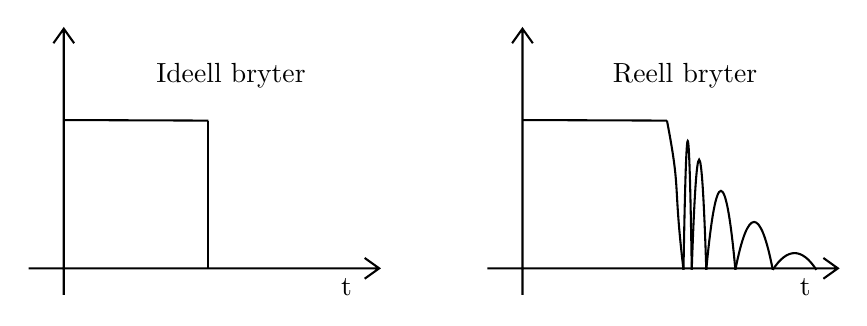
\begin{tikzpicture}[x=0.75pt,y=0.75pt,yscale=-1,xscale=1]
%uncomment if require: \path (0,300); %set diagram left start at 0, and has height of 300

%Shape: Axis 2D [id:dp9901238578898577] 
\draw  (33,170.45) -- (201.86,170.45)(49.89,55) -- (49.89,183.27) (194.86,165.45) -- (201.86,170.45) -- (194.86,175.45) (44.89,62) -- (49.89,55) -- (54.89,62)  ;
%Shape: Axis 2D [id:dp6811118948253481] 
\draw  (254,170.45) -- (422.86,170.45)(270.89,55) -- (270.89,183.27) (415.86,165.45) -- (422.86,170.45) -- (415.86,175.45) (265.89,62) -- (270.89,55) -- (275.89,62)  ;
%Straight Lines [id:da4843943952741787] 
\draw    (50,99) -- (119.5,99.27) ;
%Straight Lines [id:da293121433985875] 
\draw    (119.5,99.27) -- (119.5,170.27) ;
%Straight Lines [id:da6762241711099313] 
\draw    (271,99) -- (340.5,99.27) ;
%Shape: Parabola [id:dp5439190691797124] 
\draw   (352.45,171.11) .. controls (351.19,88.44) and (349.86,88.44) .. (348.47,171.11) ;
%Shape: Parabola [id:dp8649858969152793] 
\draw   (359.45,171.12) .. controls (357.18,100.44) and (354.84,100.44) .. (352.45,171.11) ;
%Shape: Parabola [id:dp36725763713463566] 
\draw   (373.47,171.13) .. controls (368.84,120.43) and (364.17,120.43) .. (359.45,171.12) ;
%Shape: Parabola [id:dp4674702723898885] 
\draw   (391.48,171.15) .. controls (385.5,140.42) and (379.49,140.42) .. (373.47,171.13) ;
%Shape: Parabola [id:dp8011958280177405] 
\draw   (412.49,171.16) .. controls (405.5,160.42) and (398.5,160.41) .. (391.48,171.15) ;
%Curve Lines [id:da6229326940059043] 
\draw    (340.5,99.27) .. controls (347.33,134.63) and (343.33,127.63) .. (348.47,171.11) ;

% Text Node
\draw (182,174) node [anchor=north west][inner sep=0.75pt]   [align=left] {t};
% Text Node
\draw (403,174) node [anchor=north west][inner sep=0.75pt]   [align=left] {t};
% Text Node
\draw (253,67) node [anchor=north west][inner sep=0.75pt]   [align=left] {\si{\V}};
% Text Node
\draw (33,67) node [anchor=north west][inner sep=0.75pt]   [align=left] {\si{\V}};
% Text Node
\draw (93,70) node [anchor=north west][inner sep=0.75pt]   [align=left] {Ideell bryter};
% Text Node
\draw (313,70) node [anchor=north west][inner sep=0.75pt]   [align=left] {Reell bryter};


\end{tikzpicture}}
    \caption{Spenningen over en ideell- og en reell bryter.}
    \label{fig:bryter}
\end{figure}

Stort sett er det to grunner til at dette ikke er et problem:

\begin{enumerate}
    \item Vi har tactile pushbuttons på micro:bit-en. Disse er mye bedre på å redusere bounce enn andre typer knapper.
    \item I tillegg, dersom man manuelt sjekker knappeverdien i software, vil CPU-en som oftest ikke være rask nok til å merke at transienten er der. Dette er grunnen til at dere sannsynligvis ikke hadde dette problemet da dere brukte \verb|GPIO|-modulen.
\end{enumerate}

For å komme rundt \textit{input bounce} problemet, kan man gjøre debouncing i enten software eller hardware. I hardware ville man lagt til en RC-krets til knappen, slik at spenningen blir lavpass-filtrert før micro:bit-en kan lese den. I software kan man simpelthen vente i en kort stund om man først leser en endring, slik at man hopper over transienten.

I vårt tilfelle er knappene bare trukket høye med en pullup, og det er ikke noe vi kan egentlig gjøre for å endre på det. Siden vi i denne oppgaven koblet \verb|A|-knappen direkte til LED-matrisen med \verb|GPIOTE| og \verb|PPI|, har vi heller ikke muligheten til å legge inn software debouncing uten å bryte den evige løkka vi allerede har implementert. Strengt tatt kunne vi koblet knappen fra \verb|GPIOTE| inn i en \verb|TIMER|-instans gjennom \verb|PPI|, og deretter brukt en ny \verb|PPI|-kanal til å koble en overflythendelse fra \verb|TIMER|-instansen inn på \verb|GPIOTE|-oppgavene, men dette er mye mer innsats for en marginal forbedring.

\subsection{Hint}\label{subsec:PPI-hint}


\begin{itemize}
    \item Husk å aktivere hver \verb|PPI|-kanal. Når de er konfigurert riktig, aktiveres de ved å skrive til \verb|CHENSET| i \verb|PPI|-instansen (husk at vi bare bruker seks \verb|PPI|-kanaler totalt).
    \item \verb|GPIOTE|-kanalene trenger ingen eksplisitt aktivering fordi \verb|MODE|-feltet i \verb|CONFIG|-registeret automatisk tar hånd om pinnen for dere.
\end{itemize}



ls
\section{Oppgave 4: Two Wire Interface (frivillig)}

\subsection{Beskrivelse}

En av de vanligste protokollene for seriell kommunikasjon er I2C (også formatert som I$^2$C), som står for \textbf{I}nter-\textbf{I}ntegrated \textbf{C}ircuit. Denne protokollen ble utviklet av Philips Semiconductor (i dag NXP Semiconductors), som låste ned protokollen bak en del registrerte varemerker.

Av den grunn, begynte andre produsenter å implementere protokollen under andre navn, hvor den mest brukte er \verb|TWI| (\textbf{T}wo \textbf{W}ire \textbf{I}nterface). Siden 2006 kreves det ikke lenger lisens for å implementere I2C under navnet I2C, man man kommer fortsatt over navn som stort sett er synonyme (se forøvrig forelesningsvideoer for mer informasjon om I2C).

I Nordic sitt tilfelle, implementerer nRF52-serien et supersett av I2C; den vanlige protokollen har støtte for vanlig rate på 100 kbps og \textit{Fast-mode} (400 kbps). I tillegg støtter også nRFen også et mellommodus på 250 kbps.

Det dere skal gjøre i denne oppgaven, er å bruke \verb|TWI|-bussen til nRF52833-SoCen til å kommunisere med akselerometeret som finnes på micro:bit-en. Dere skal deretter bruke denne sensorinformasjonen til å lyse opp en LED i matrisen basert på hvordan micro:bit-en er orientert.

For de mest interesserte, så finner dere et lite appendiks om I2C i appendiks \ref{app:TWI}.

Uheldigvis så er jeg ennå ikke ferdig med denne oppgaven, men den vil bli gitt ut på BlackBoard snarest mulig.

% \subsection{Oppgave - Grunnleggende TWI-kommunikasjon}

% Først og fremst må dere finne ut hvordan akselerometeret er koblet til nRFen. Et naturlig sted å starte er \verb|schematic.pdf|. Det dere skal se etter er pinnene kalt \verb|SDA| (\textbf{S}erial \textbf{D}ata) og SCL (\textbf{S}erial \textbf{C}lock). Dette er de to linjene som utjgør \verb|TWI|-bussen.

% Etter dette, må man finne ut hva akselerometeret forventer skal skje på \verb|TWI|-bussen. Dette er beskrevet i databladet \verb|"MMA8653FC.pdf"|, under seksjon 5.8. Det viktige er at dere vet hvilken adresse akselerometeret har, og hvordan man leser ett- og flere byte. Et lite hint er å ikke grave dere ned i detaljer; prøv å få et overblikk først. For eksempel; om dere ikke vet hva en \textit{start condition} er, så er det nok å vite at nRFen lager en for dere. Om dere allikevel vil vite litt mer om I2C, så kan dere referere til appendiks \ref{app:TWI} for å lese mer om protokollen, eventuelt se forelesningene som omhandler temaet.


% \cprotect\subsubsection{\lstinline{void twi_init()}}

% Det første som må gjøres er å lage filene \verb|twi.h| og \verb|twi.c|.

% \begin{itemize}
%     \item I headerfilen deklarerer dere funksjonen \verb|void twi_init()|. Den tilhørende implementasjonen skal aktivere \verb|TWI|-modulen på nRFen med de riktige signallinjene og 100 kbps overføringshastighet. Legg merke til at signallinjene først må konfigureres av \verb|GPIO|-modulen. Dette er beskrevet i referansemanualen, under seksjon 6.27. 
% \end{itemize}

% Som før, må dere først lage en \verb|struct| som mapper ut adresseområdet til \verb|TWI|-modulen:


% \begin{lstlisting}
% #define TWI0 ((NRF_TWI_REG*)__TWI_BASE_ADDRESS__)

% typedef struct {
%         volatile uint32_t TASKS_STARTRX;
%         [...]
% } NRF_TWI_REG;
% \end{lstlisting}

% Denne \verb|struct|en er litt større enn det \verb|UART|-\verb|struct|-en fra tidligere er. Riktige verdier for de reserverte områdene er oppgitt i hintene, men prøv først å finne dem selv.




% \cprotect\subsubsection{\lstinline{void twi_multi_read()}}

% Som dere kan se i appendiks \ref{app:TWI} og i databladet til akselerometeret, er det mulig å lese- eller skrive flere byte om gangen, uten å måtte gi fra seg \verb|TWI|-bussen. Dette er også mer effektivt, fordi man slipper å sende slavens adresse på nytt for hver byte. Måten I2C-enheter gjør dette på, er at de automatisk hopper til et nytt internt register hver gang du har lest fra- eller skrevet til et (sjekk databladet!).

% Istedenfor å lage funksjoner som leser- og skriver ett og ett register, skal vi lage mer generelle funksjoner som kan lese- og skrive \textit{n} registre av gangen. Vi kan da simpelthen sette \textit{n} lik \verb|1| om vi trenger kun ett. 
% Start med å legge denne deklarasjonen i \verb|twi.h|:

% \begin{lstlisting}
% void twi_multi_read(
%         uint8_t slave_address,
%         uint8_t start_register,
%         int registers_to_read,
%         uint8_t * data_buffer
%         );
% \end{lstlisting}


% Siden vi bruker typen \verb|uint8_t|, må vi nå inkludere \verb|<stdint.h>| i \verb|twi.h|. Med denne koden ønsker vi at det følgende skal skje:
% \begin{enumerate}
%     \item Først skal vi kunne adressere en vilkårlig slave, med adresse \verb|slave_address|.
%     \item  Deretter skal vi fortelle slaven hvilket register vi ønsker å begynne å lese fra. I dette tilfellet er det \verb|start_register|.
%     \item Når dette er gjort, skal vi lese så mange byte vi trenger (\verb|registers_to_read|), og putte dem i arrayet \verb|data_buffer|.
%     \item Til slutt avslutter vi kommunikasjonen og forlater \verb|TWI|-bussen.
% \end{enumerate}

% Seksjon 28.6 i nRF51-databladet forklarer veldig godt hvordan dette skal gjøres. Her har dere en oppsummering av hva som skal til:


% \begin{enumerate}
%     \item Sett \verb|ADDRESS|-registeret til \verb|slave_address|.
%     \item Start en skriveoperasjon.
%     \item Når dere har fått \verb|ACK| tilbake fra slaven (som betyr at en \verb|TXDSENT|-hendelse er blitt generert), starter dere en leseoperasjon uten å stoppe bussen. Dette kalles en repeated start sequence.
%     \item Les \verb|TWI|-bussen (r\verb|registers_to_read -1|) ganger. Dette er fordi dere må sende en \verb|NACK| til slaven den siste gangen dere leser en byte. Hver verdi dere leser, dytter dere inn i \verb|data_buffer|. 
%     \item Til slutt kjører dere \verb|STOP|-oppgaven, før dere leser busser for siste gang. Dette vil gjøre at nRFen generer en \verb|NACK| istedenfor en \verb|ACK|, slik at slaven ikke sender ut flere byte på bussen.
% \end{enumerate}

% Hendelsen \verb|TXDSENT| settes ikke automatisk til \verb|0| når dere dytter en ny byte inn i \verb|TXD|. Det samme gjelder også for \verb|RXDREADY|-registeret. Derfor er det nødvendig å gjøre dette manuelt:

% \begin{lstlisting}
% TWI0->TXDSENT = 0;
% TWI0->TXD = start_register;
% while(!TWI0->TXDSENT);

% [...]

% TWI0->RXDREADY = 0;
% TWI0->STARTRX = 1;
% \end{lstlisting}

% For å prøve ut \verb|void twi_multi_read(...)| skal vi forsøke å lese akselerometerets enhets-ID. Denne ligger lagret i et register kalt \verb|WHO_AM_I|. Adressen til dette registeret finner dere i seksjon 6 i databladet til akselerometeret.

% Siden vi er kun ute etter en byte, holder det å ta pekeren til \verb|uint8_t| og bruke det som en buffer for å dytte ID-en inn i. Men for å gjøre det mer generelt til senere, skal vi bruke \verb|malloc()| (fra biblioteket \verb|<stdlib.h>|), som har samme funksjon som \verb|new| i C++. For å allokere minne kan dere gjøre noe slikt:


% \begin{lstlisting}
% uint8_t * data_buffer;
% data_buffer = (uint8_t *)malloc(8 * sizeof(uint8_t));

% [...]

% free(data_buffer);
% \end{lstlisting}

% Dette vil allokere minne til et dynamisk array av 8 \verb|uint8_t|, hvor \verb|free| i C brukes for å frigi dynamisk allokert minne tilbake til heapen.

% For å teste om \verb|TWI|-bussen fungerer, kan dere sammenligne det dere får tilbake med akselerometerets fabrikk-ID; \verb|0x5A|, eller 90 i base 10. Om dette er det dere får, kan dere for eksempel skru på LED-matrisen, eller sende en melding over \verb|UART| for å signalisere at ting virker som det skal.


% \cprotect\subsubsection{\lstinline{void twi_multi_write()}}

% Å skrive \verb|n| byte til en vilkårlig slave er mye lettere enn å lese. Grunnen til dette er at når vi skriver data, så trenger vi ikke å ta hensyn til NACK-grensetilfellet fra leseoperasjonen. 

% Til og starte med legger dere til denne deklarasjonen i \verb|twi.h|:

% \begin{lstlisting}
% void twi_multi_write(
%         uint8_t slave_address,
%         uint8_t start_register,
%         int registers_to_write,
%         uint8_t * data_buffer
%         );
% \end{lstlisting}

% Sekvensen vi trenger å implementere er beskrevet i seksjon 28.5 i nRF52-databladet. Kort fortalt skal dere:

% \begin{enumerate}
%     \item Sette \verb|ADRESS|-registeret.
%     \item Starte en skriveoperasjon
%     \item Skrive \verb|registers_to_write| antall byte til bussen
%     \item Kalle \verb|STOP|-oppgaven.
% \end{enumerate}

% Som før, må vi huske å manuelt sette \verb|TXDSENT| til 0 etter at hendelsen er blitt aktivert:


% \begin{lstlisting}
% [...]

% TWI0->TXDSENT = 0;
% TWI0->TXD = data_buffer[n];
% while(!TWI0->TXDSENT);

% [...]

% \end{lstlisting}

% \subsection{Oppgave - Lesing av akselerometeret}

% Når dere har skrevet både \verb|twi_multi_read| og \verb|twi_multi_write|, kan disse brukes til å lese akselerometerets \verb|x-, y-,| og \verb|z|-registre. For å slippe å kalle \verb|TWI|-spesifikke funksjoner direkte fra \verb|main|, har dere allerede fått utlevert en wrapper for akselerometeret, som bruker \verb|TWI|-funksjonene dere allerede har skrevet. Denne heter \verb|accel.h|, og deklarer funksjonene \verb|void accel_init()| og \verb|void accel_read_x|\newline\verb|_y_z(int * data_buffer)|.   


% Funksjonen \verb|accel_init()| vil skru akselerometeret på, og sette oppdateringsraten til 200 Hz. Denne funksjonen krever at \verb|TWI|-bussen er initialisert i forkant. 

% Funksjonen \verb|accel_read_x_y_z(int * data_buffer)| tar inn en peker til et array av typen \verb|int|. Dette arrayet må minst være av størrelse 3, hvis ikke risikerer man uforutsigbar oppførsel. Det har derimot ikke noe å si om arrayet er større enn 3. Når funksjonen er kjørt ferdig, vil de tre første elementene i dette arrayet være henholdsvis \verb|x-, y-,| og \verb|z-|komponentene til akselerasjonen som akselerometeret måler. Se figur \ref{fig:4-høyrehåndskoordinatsystemet} for å se koordinatsystemet dere får komponentene i.

% \subsubsection{Fyll inn konstanter i \texttt{accel.c}}

% Før dere kan bruke funksjonene i \verb|accel.h|, må dere fylle ut tre verdier i implementasjonsfilen \verb|accel.c|:


% \begin{itemize}
%     \item \verb|ACCEL_ADDR| er adressen til akselerometeret, som dere fant i databladet\newline \verb|"MMA8653.pdf"| under seksjon 5.8.
%     \item \verb|ACCEL_DATA_REG| er adressen til det mest signifikante bytet av akselerometerets x-komponent. Dette kan dere finne under seksjon 6 i databladet.
%     \item \verb|ACCEL_CTRL_REG_1| er adressen til registeret som kontroller dataraten, og om akselerometeret er på eller ei. Dette kan også finnes under seksjon 6 i databladet.
% \end{itemize}

% \begin{figure}[ht]
%     \centering
    


% \tikzset{every picture/.style={line width=0.75pt}} %set default line width to 0.75pt        

% \resizebox{.45\textwidth}{!}{\begin{tikzpicture}[x=0.75pt,y=0.75pt,yscale=-1,xscale=1]
% %uncomment if require: \path (0,300); %set diagram left start at 0, and has height of 300

% %Rounded Rect [id:dp0932893899360494] 
% \draw   (100,56) .. controls (100,39.43) and (113.43,26) .. (130,26) -- (250,26) .. controls (266.57,26) and (280,39.43) .. (280,56) -- (280,146) .. controls (280,162.57) and (266.57,176) .. (250,176) -- (130,176) .. controls (113.43,176) and (100,162.57) .. (100,146) -- cycle ;
% %Straight Lines [id:da3951030214501392] 
% \draw    (72,101) -- (190,101) ;
% \draw [shift={(70,101)}, rotate = 0] [color={rgb, 255:red, 0; green, 0; blue, 0 }  ][line width=0.75]    (10.93,-3.29) .. controls (6.95,-1.4) and (3.31,-0.3) .. (0,0) .. controls (3.31,0.3) and (6.95,1.4) .. (10.93,3.29)   ;
% %Straight Lines [id:da13155371681429218] 
% \draw    (190,204) -- (190,101) ;
% \draw [shift={(190,206)}, rotate = 270] [color={rgb, 255:red, 0; green, 0; blue, 0 }  ][line width=0.75]    (10.93,-3.29) .. controls (6.95,-1.4) and (3.31,-0.3) .. (0,0) .. controls (3.31,0.3) and (6.95,1.4) .. (10.93,3.29)   ;
% %Straight Lines [id:da0863339023239853] 
% \draw    (239.59,51.41) -- (190,101) ;
% \draw [shift={(241,50)}, rotate = 135] [color={rgb, 255:red, 0; green, 0; blue, 0 }  ][line width=0.75]    (10.93,-3.29) .. controls (6.95,-1.4) and (3.31,-0.3) .. (0,0) .. controls (3.31,0.3) and (6.95,1.4) .. (10.93,3.29)   ;
% %Straight Lines [id:da6196325519456647] 
% \draw  [dash pattern={on 4.5pt off 4.5pt}]  (190,101) -- (157,134) ;
% %Shape: Square [id:dp7211777686672174] 
% \draw  [fill={rgb, 255:red, 0; green, 0; blue, 0 }  ,fill opacity=1 ] (123,45) -- (149,45) -- (149,71) -- (123,71) -- cycle ;
% %Shape: Square [id:dp6606801844368411] 
% \draw  [fill={rgb, 255:red, 11; green, 11; blue, 11 }  ,fill opacity=1 ] (234,64) -- (251,64) -- (251,81) -- (234,81) -- cycle ;

% % Text Node
% \draw (167,136) node [anchor=north west][inner sep=0.75pt]   [align=left] {micro:bit};
% % Text Node
% \draw (217,39) node [anchor=north west][inner sep=0.75pt]   [align=left] {Z};
% % Text Node
% \draw (63,106) node [anchor=north west][inner sep=0.75pt]   [align=left] {X};
% % Text Node
% \draw (197,199) node [anchor=north west][inner sep=0.75pt]   [align=left] {Y};


% \end{tikzpicture}}
%     \caption{Høyrehåndskoordinatsystemet \texttt{accel\_read\_x\_y\_z} bruker.}
%     \label{fig:4-høyrehåndskoordinatsystemet}
% \end{figure}


% \subsection{Oppgave - Skriv verdier til skjerm med UART}

% Når dere har fylt inn konstantene i \verb|accel.c|, er det fritt frem for å bruke funksjonene filen definerer. For å gjøre det lettere å skrive til skjermen, har dere også fått utlevert \verb|utility.h| med tilhørende implementasjonsfil. Denne filen gir dere funksjonen \verb|utility_print|, som etterligner funksjonaliteten til \verb|printf|, uten å trekke inn for mye annet som \verb|<stdio.h>| bringer med seg.


% Det er opp til dere om dere vil bruke \verb|utility_print|, men her er et eksempel på hvordan funksjonen kan brukes (se \verb|utility.h|):



% \begin{lstlisting}
% int * data_buffer = (int *)malloc(3 * sizeof(int));
% accel_read_x_y_z(data_buffer);

% int x_acc = data_buffer[0];
% int y_acc = data_buffer[1];
% int z_acc = data_buffer[2];

% utility_print(&uart_send, "X: %6d Y: %6d Z: %6d\n\r", x_acc,
% -> y_acc, z_acc);
% \end{lstlisting}

% \subsection{Oppgave - Lys opp riktig diode}

% Når dere greier å lese fra akselerometeret, er det på tide å ha det litt gøy med LED-matrisen til micro:bit-en. På grunn av måten matrisen er koblet opp på, er det litt komplisert å skru på en og en diode. For å gjøre det litt enkelt, har dere fått utlevert filen \verb|ubit_led_matrix.h|, som dere er mer enn velkomne til å benytte dere av. Et forslag til hvordan denne brukes, ser slik ut:



% \begin{lstlisting}
% ubit_led_matrix_init();

% [...]

% // Calculate X-LED and Y-LED from accelerometer reading

% ubit_led_matrix_light_only_at(x_led, y_led);
% \end{lstlisting}

% Koordinatsystemet \verb|ubit_led_matrix_light_only_at(int x, int y)| bruker, er illustrert i figur \ref{fig:4-coordinate} Hvordan dere regner ut hvilke koordinater som skal lyse opp gitt akselerasjonen i \verb|x-| og \verb|y-|retning, er opp til dere. Et eksempel på hvordan dette kan gjøres kan dere se her:



% \begin{lstlisting}
% int x_accel = data_buffer[0];
% int y_accel = data_buffer[1];

% int x_dot = x_accel / 50;
% int y_dot = - y_accel / 50;

% ubit_led_matrix_light_only_at(x_dot, y_dot);
% \end{lstlisting}




% \subsection{Oppgave 4 - Lesing av magnetometeret (Frivilig)}

% Med \verb|void twi_multi_read(...)| og \verb|void twi_multi_write(...) | er det ganske lett å lese fra magnetometeret også. Dette gjøres på samme måte som for akselerometeret, og er beskrevet i databladet \verb|"MAG3110.pdf"|. Noe som er kult å implementere er å prøve å bruke magnetometeret som et kompass.



% \subsection{Hint}\label{subsec:TWI-hint}

% \begin{itemize}
%     \item Verdier for de 15 reserverte områdene: 1, 2, 1, 56, 4, 1, 4, 49, 63, 110, 14, 1, 2, 1, 24.
%     \item nRF51822en har to instanser av \verb|TWI|-modulen, som betyr at dere kan ha to forskjellige \verb|TWI|-linjer oppe på en gang. Vi trenger bare en av dem i labben.
%     \item Husk å manuelt sette \verb|RXREADY| og \verb|TXDSENT| til \verb|0| etter at dere sjekker disse registrene.
%     \item Det er egentlig unødvendig å bruke dynamisk minne i denne oppgaven. Siden vi vet ved kompileringstiden hvor stor plass vi trenger, kan vi simpelthen opprette en vanlig liste. Vi bruker dynamisk minne bare for å eksponere dere til C-ekvivalenten av \verb|new|.
%     \item Hver gang dere kaller \verb|make flash|, tilbakestilles bare nRFen på micro:bit-en. Akselerometeret og magnetometeret lever helt sine egne liv. Det betyr at om dere sender en feilaktig \verb|TWI|-melding, kan dere sette disse i en tilstand hvor ikke svarer på korrekte \verb|TWI|-meldinger senere. Om koden deres ser riktig ut, men ting fortsatt ikke fungerer, kan dette være årsaken. Løsningen er rett og slett å ta strømmen og prøve på nytt,
% \end{itemize}

% \begin{figure}[ht]
%     \centering
    

% \tikzset{every picture/.style={line width=0.75pt}} %set default line width to 0.75pt        

% \resizebox{.55\textwidth}{!}{\begin{tikzpicture}[x=0.75pt,y=0.75pt,yscale=-1,xscale=1]
% %uncomment if require: \path (0,300); %set diagram left start at 0, and has height of 300

% %Shape: Square [id:dp8233412643298406] 
% \draw   (178.33,41) -- (214.33,41) -- (214.33,77) -- (178.33,77) -- cycle ;
% %Straight Lines [id:da04978765244805894] 
% \draw    (178.33,34) -- (376.33,34) ;
% \draw [shift={(378.33,34)}, rotate = 180] [color={rgb, 255:red, 0; green, 0; blue, 0 }  ][line width=0.75]    (10.93,-3.29) .. controls (6.95,-1.4) and (3.31,-0.3) .. (0,0) .. controls (3.31,0.3) and (6.95,1.4) .. (10.93,3.29)   ;
% %Straight Lines [id:da5810221223288496] 
% \draw    (171.33,43) -- (171.33,241) ;
% \draw [shift={(171.33,41)}, rotate = 90] [color={rgb, 255:red, 0; green, 0; blue, 0 }  ][line width=0.75]    (10.93,-3.29) .. controls (6.95,-1.4) and (3.31,-0.3) .. (0,0) .. controls (3.31,0.3) and (6.95,1.4) .. (10.93,3.29)   ;
% %Shape: Square [id:dp5059092724274146] 
% \draw   (178.33,82) -- (214.33,82) -- (214.33,118) -- (178.33,118) -- cycle ;
% %Shape: Square [id:dp2891912933808465] 
% \draw   (219.33,41) -- (255.33,41) -- (255.33,77) -- (219.33,77) -- cycle ;
% %Shape: Square [id:dp1645770762275951] 
% \draw   (219.33,82) -- (255.33,82) -- (255.33,118) -- (219.33,118) -- cycle ;
% %Shape: Square [id:dp9736278568511694] 
% \draw   (178.33,123) -- (214.33,123) -- (214.33,159) -- (178.33,159) -- cycle ;
% %Shape: Square [id:dp029867780453355364] 
% \draw   (178.33,164) -- (214.33,164) -- (214.33,200) -- (178.33,200) -- cycle ;
% %Shape: Square [id:dp12476991182906527] 
% \draw   (219.33,123) -- (255.33,123) -- (255.33,159) -- (219.33,159) -- cycle ;
% %Shape: Square [id:dp7528475341079031] 
% \draw   (219.33,164) -- (255.33,164) -- (255.33,200) -- (219.33,200) -- cycle ;
% %Shape: Square [id:dp1831693275579498] 
% \draw   (260.33,41) -- (296.33,41) -- (296.33,77) -- (260.33,77) -- cycle ;
% %Shape: Square [id:dp29795524177828026] 
% \draw   (260.33,82) -- (296.33,82) -- (296.33,118) -- (260.33,118) -- cycle ;
% %Shape: Square [id:dp4122946314436253] 
% \draw   (301.33,41) -- (337.33,41) -- (337.33,77) -- (301.33,77) -- cycle ;
% %Shape: Square [id:dp5406864507250528] 
% \draw   (301.33,82) -- (337.33,82) -- (337.33,118) -- (301.33,118) -- cycle ;
% %Shape: Square [id:dp7175399457747331] 
% \draw   (260.33,123) -- (296.33,123) -- (296.33,159) -- (260.33,159) -- cycle ;
% %Shape: Square [id:dp10310365620490436] 
% \draw   (260.33,164) -- (296.33,164) -- (296.33,200) -- (260.33,200) -- cycle ;
% %Shape: Square [id:dp49927602057398457] 
% \draw   (301.33,123) -- (337.33,123) -- (337.33,159) -- (301.33,159) -- cycle ;
% %Shape: Square [id:dp5344360980187939] 
% \draw   (301.33,164) -- (337.33,164) -- (337.33,200) -- (301.33,200) -- cycle ;
% %Shape: Square [id:dp8773632673124938] 
% \draw   (342.33,41) -- (378.33,41) -- (378.33,77) -- (342.33,77) -- cycle ;
% %Shape: Square [id:dp6452173632136904] 
% \draw   (342.33,82) -- (378.33,82) -- (378.33,118) -- (342.33,118) -- cycle ;
% %Shape: Square [id:dp009772691508731945] 
% \draw   (342.33,123) -- (378.33,123) -- (378.33,159) -- (342.33,159) -- cycle ;
% %Shape: Square [id:dp9249607675718099] 
% \draw   (342.33,164) -- (378.33,164) -- (378.33,200) -- (342.33,200) -- cycle ;
% %Shape: Square [id:dp08207948183332348] 
% \draw   (178.33,205) -- (214.33,205) -- (214.33,241) -- (178.33,241) -- cycle ;
% %Shape: Square [id:dp3655157745108586] 
% \draw   (219.33,205) -- (255.33,205) -- (255.33,241) -- (219.33,241) -- cycle ;
% %Shape: Square [id:dp8902660214680873] 
% \draw   (260.33,205) -- (296.33,205) -- (296.33,241) -- (260.33,241) -- cycle ;
% %Shape: Square [id:dp09583767081953454] 
% \draw   (301.33,205) -- (337.33,205) -- (337.33,241) -- (301.33,241) -- cycle ;
% %Shape: Square [id:dp00012445236088143297] 
% \draw   (342.33,205) -- (378.33,205) -- (378.33,241) -- (342.33,241) -- cycle ;

% % Text Node
% \draw (270,13) node [anchor=north west][inner sep=0.75pt]   [align=left] {$\displaystyle X$};
% % Text Node
% \draw (155,135) node [anchor=north west][inner sep=0.75pt]   [align=left] {$\displaystyle Y$};
% % Text Node
% \draw (181,53) node [anchor=north west][inner sep=0.75pt]  [font=\scriptsize] [align=left] {(-2,2)};
% % Text Node
% \draw (222,53) node [anchor=north west][inner sep=0.75pt]  [font=\scriptsize] [align=left] {(-1,2)};
% % Text Node
% \draw (265,53) node [anchor=north west][inner sep=0.75pt]  [font=\scriptsize] [align=left] {(0,2)};
% % Text Node
% \draw (306,53) node [anchor=north west][inner sep=0.75pt]  [font=\scriptsize] [align=left] {(1,2)};
% % Text Node
% \draw (347,53) node [anchor=north west][inner sep=0.75pt]  [font=\scriptsize] [align=left] {(2,2)};
% % Text Node
% \draw (181,93) node [anchor=north west][inner sep=0.75pt]  [font=\scriptsize] [align=left] {(-2,1)};
% % Text Node
% \draw (222,93) node [anchor=north west][inner sep=0.75pt]  [font=\scriptsize] [align=left] {(-1,1)};
% % Text Node
% \draw (265,93) node [anchor=north west][inner sep=0.75pt]  [font=\scriptsize] [align=left] {(0,1)};
% % Text Node
% \draw (306,93) node [anchor=north west][inner sep=0.75pt]  [font=\scriptsize] [align=left] {(1,1)};
% % Text Node
% \draw (347,93) node [anchor=north west][inner sep=0.75pt]  [font=\scriptsize] [align=left] {(2,1)};
% % Text Node
% \draw (181,134) node [anchor=north west][inner sep=0.75pt]  [font=\scriptsize] [align=left] {(-2,0)};
% % Text Node
% \draw (222,134) node [anchor=north west][inner sep=0.75pt]  [font=\scriptsize] [align=left] {(-1,0)};
% % Text Node
% \draw (265,134) node [anchor=north west][inner sep=0.75pt]  [font=\scriptsize] [align=left] {(0,0)};
% % Text Node
% \draw (306,134) node [anchor=north west][inner sep=0.75pt]  [font=\scriptsize] [align=left] {(1,0)};
% % Text Node
% \draw (347,134) node [anchor=north west][inner sep=0.75pt]  [font=\scriptsize] [align=left] {(2,0)};
% % Text Node
% \draw (179,175) node [anchor=north west][inner sep=0.75pt]  [font=\scriptsize] [align=left] {(-2,-1)};
% % Text Node
% \draw (220,175) node [anchor=north west][inner sep=0.75pt]  [font=\scriptsize] [align=left] {(-1,-1)};
% % Text Node
% \draw (263,175) node [anchor=north west][inner sep=0.75pt]  [font=\scriptsize] [align=left] {(0,-1)};
% % Text Node
% \draw (304,175) node [anchor=north west][inner sep=0.75pt]  [font=\scriptsize] [align=left] {(1,-1)};
% % Text Node
% \draw (345,176) node [anchor=north west][inner sep=0.75pt]  [font=\scriptsize] [align=left] {(2,-1)};
% % Text Node
% \draw (179,216) node [anchor=north west][inner sep=0.75pt]  [font=\scriptsize] [align=left] {(-2,-2)};
% % Text Node
% \draw (220,216) node [anchor=north west][inner sep=0.75pt]  [font=\scriptsize] [align=left] {(-1,-2)};
% % Text Node
% \draw (263,216) node [anchor=north west][inner sep=0.75pt]  [font=\scriptsize] [align=left] {(0,-2)};
% % Text Node
% \draw (304,216) node [anchor=north west][inner sep=0.75pt]  [font=\scriptsize] [align=left] {(1,-2)};
% % Text Node
% \draw (345,216) node [anchor=north west][inner sep=0.75pt]  [font=\scriptsize] [align=left] {(2,-2)};




% % Text Node
% \draw (177,634) node [anchor=north west][inner sep=0.75pt]  [font=\large] [align=left] {\texttt{P28}};
% % Text Node
% \draw (228,634) node [anchor=north west][inner sep=0.75pt]  [font=\large] [align=left] {\texttt{P11}};
% % Text Node
% \draw (277,634) node [anchor=north west][inner sep=0.75pt]  [font=\large] [align=left] {\texttt{P31}};
% % Text Node
% \draw (332,634) node [anchor=north west][inner sep=0.75pt]  [font=\large] [align=left] {\texttt{P5}};
% % Text Node
% \draw (378,634) node [anchor=north west][inner sep=0.75pt]  [font=\large] [align=left] {\texttt{P30}};
% % Text Node
% \draw (426,395) node [anchor=north west][inner sep=0.75pt]  [font=\large] [align=left] {\texttt{P21 (ROW 1)}};
% % Text Node
% \draw (426,445) node [anchor=north west][inner sep=0.75pt]  [font=\large] [align=left] {\texttt{P22 (ROW 2)}};
% % Text Node
% \draw (426,495) node [anchor=north west][inner sep=0.75pt]  [font=\large] [align=left] {\texttt{P15 (ROW 3)}};
% % Text Node
% \draw (157,341.4) node [anchor=north west][inner sep=0.75pt]   [align=left] {Implementasjon i hardware (LED matrise)};
% % Text Node
% \draw (426,545) node [anchor=north west][inner sep=0.75pt]  [font=\large] [align=left] {\texttt{P24 (ROW 4)}};
% % Text Node
% \draw (426,595) node [anchor=north west][inner sep=0.75pt]  [font=\large] [align=left] {\texttt{P19 (ROW 5)}};




% \end{tikzpicture}}
%     \caption{Koordinatsystemet \texttt{ubit\_led\_matrix\_light\_only\_at} bruker.}
%     \label{fig:4-coordinate}
% \end{figure}    


% \section{Oppgave 5: BLE GAP}

% \subsection{Beskrivelse}
% BLE (\textbf{B}luetooth \textbf{L}ow \textbf{E}nergy), og er versjon 4.2 av Bluetoothspesifikasjonen. I appendiks \ref{app:ble} kan dere lese litt mer om Bluetooth 4.2, og forskjellene fra Bluetooth Classic. Denne oppgaven er derimot ganske selvinnskapslet, så det er ikke noe krav å ha omfattende kjennskap til spesifikasjonen. Det er forøvrig ikke sunt å ha omfattende kjennskap til spesifikasjonen heller - med tanke på at siste utgave av kjernespesifikasjonen heller - med tanke på at siste utgave av kjernespesifikasjonen alene (bluetooth.com) er på rolige 3000 sider.

% \subsubsection{Testing}

% For å koble til micro:bit-en over Bluetooth skal vi bruke "nRF Connect", som er en app dere kan laste ned fra Google Play eller Appstore. Det er utlevert et eksempelprogram, kalt \verb|example.hex| som dere kan flashe til micro:bit-en for å teste. Det gjøres ved å kalle:

% \verb|nrfjprog -f nrf51 --chiperase --program example.hex --reset|

% Når dere åpner nRF COnnect vil telefonen deres starte å skanne etter advertising packets (se figur ....). For å begrense antall enheter som vises kan dere sette RSSI-filteret, som bestemmer minimal signalstyrke før en enhet vises. I figur ... er filteret satt til -80 dBm. På Sanntidssalen vil det være mange andre enheter i nærheten, så en verdi nærmere -60 dBm er muligens bedre.

% Når dere kobler til micro:bit-en vil dere se noe som minner om figur ... Navnene "Led Matrix" og "Buttons" vil ikke vises i første omgang, men dere kan selv sette dem ved å trykke lenge på characteristics og redigere navnet. Navnet på karakteristikken er kun kosmetisk, og påvirker ikke hvordan micro:bit-en oppfører seg.

% Ved å laste opp et byte forskjellig fra \verb|0x00| til karakteristikken "Led Matrix" vil LED-matrisn skru seg på. Ved å laste opp bytet \verb|0x00| vil matrisen skru seg av igjen.

% Karaktereristikken kalt "Buttons" inneholder informasjon om tilstanden til knappene på micro:bit-en. Dere kan lese denne verdien en gang ved å trykke nedlastingsikonet; eller dere kan subscribe til karakteristikken ved å trykke "notifikasjonsikonet" (heltrukken linje med tre piler som peker ned). Når notifikasjoner er på, vil telefonen automatisk få beskjed når dere trykker eller slipper knappene på micro:bit-en.



% \subsubsection{Kort om BLE GAP}

% Selve portvokteren i Bluetooth er kalt GAP (\textbf{G}eneric \textbf{A}ccess \textbf{P}rofile). Dette er delen av bluetooth som håndterer kringkasting, oppdagelse av enheter, oppsetting av koblinger, og etablering av sikkerhetsnivåer. 

% Selv om GAP er involvert i å etablere kobliner, er GAP i seg selv koblingsløst, og er egentlig ganske simpelt. Essensen er denne: Når du kringkaster, vil en BLE-enhet sende ut \textit{advertising packets} på 31 byte til alle som hører på, med et intervall som kan ligge mellom 20 \si{\milli\s} og 10.24 \si{\s}.

% I tillegg til dette kan envher enhet som mottar en \textit{advertising packet} forespørre mer informasjon i form av en \textit{scan request}. Når enheten som kringkaster mottar en \textit{scan request} kan den sende tilbake en \textit{scan response packet}, som også er på 31 byte. Enheten er ikke pålagt å svare på \textit{scan request}.

% GAP skjer utelukkende på kanalene 37, 38 og 39, som er reservert for kringkasting (se figur ... under appendiks ...). Grunnen til at disse kanalene er valgt for kringkasting er at de redusere mengden interferens fra WiFi, som påvirker kanalene 0-9, 11-20, og 23-32 mest.

% Det er mange måte å kringkaste på. Nyansene mellom måtene man kan sende ut \textit{advertising packets} på er ikke viktige for oss, men de er listet her opp for spesielt interesserte:

% \begin{enumerate}
%     \item \verb|ADV_IND|: "Connectable undirected advertising". Dette er den vanlige måte å sende over GAP på. Enhver annen enhet kan be om en \textit{scan response} eller en tilkobling.
%     \item \verb|ADV_DIRECT_IND|: "Connectable directed advertising". Dette brukes for å be en enhet i \textit{central mode} om en tilkobling. Denne pakken vil også kringkastes, men andre enheter som skanner vil ignorere den hvis forespurt adresse ikke samsvarer med deres egen. Enheten som sender denne pakken vil også ignorere alle \textit{scan requests}.
%     \item \verb|ADV_SCAN_IND|: "Scannable undirected advertising". Kringkasteren vil ignorere et hvert forsøk på å etablere en kobling, men kan velge å svare på \textit{scan requests}.
%     \item \verb|ADV_NONCONN_IND|: "NOn-connectable undirected advertising". Dette er modien brukt av "Bluetooth Beacons". Informasjon sende ut i hver \textit{advertising packet}, men kringkasteren vil ignorere alle forsøk på å etablere en kobling, og vil heller ikke svare på \textit{scan requests}.
% \end{enumerate}

% \subsubsection{Pakkeformat}

% Som sagt består hver \textit{advertising packet} og hver \textit{response packet} av 31 byte. Hver pakke er arrangert i et format kalt "AD Structs" - eller "Advertising Data Structures", som introduserer litt overhead. Dette gjør at vi har mindre data å gå på. Stort sett bruker man ikke GAP til å gjøre noen betydelig dataoverføring, så dette pleier ikke å være et problem.

% For å være helt korrekte, kan en kringkaster faktisk sende opp til 47 byte hvert kringkastingsintervall, men mye av dette har vi ikke kontroll over (se figur ....). Feltene som kun inneholder tall indikerer data som GAP vil sette inn, og som ikke er av interesse for oss. Vi har altså kun de 31 bytene i "Advertising Data" å bruke - og disse må struktureres i et format som spiser ytterlige 2 byte for hvert felt vi spesifiserer.

% Selv om vi ikke fult får brukt de 31 bytene vi har tilgjengelig, må vi fortsatt spesifisere hvor mange av dem vi bruker, og hvordan de er satt opp. Koden som definerer hver kringkastingspakke i eksempelprogrammet er gjengitt i kodesnutt nedenfor:


% \begin{lstlisting}
% static uint8_t adv_data[] = {
%         6, BLE_GAP_AD_TYPE_COMPLETE_LOCAL_NAME,
%         'u', ':', 'b', 'i', 't',
%         3, BLE_GAP_AD_TYPE_16BIT_SERVICE_UUID_COMPLETE,
%         0x0D, 0xF0
% };
% uint8_t adv_data_length = 11;

% \end{lstlisting}

% Det er viktig å legge merke til at vi ikke trenger å fylle ut alle 31 bytene. Dette er bevisst en del av Bluetooth 4.2 spesifikasjonen, og lar oss sende færre enn 47 byte over lufta om vi ikke har noe viktig å meddele. Dette reduserer strømforbruket til mikrokontrolleren.



% \subsection{Oppgave - Grunnleggende BLE GAP}

% Dere har fått utdelt noen C-filer som dere kan bygge på. I main vil dere set et kall til \verb|bluetooth_init()|. Dette er en wrapper rundt noen lavnivå-funksjoner som først starter Nordic sin S130 SoftDevice, for deretter å sette op BLE-stakken med noen fornuftige startparametre. Deres oppgave er å implementere funksjonen \verb|bluetooth_gap_advertising_Start()|, som er ansvarlig for å sette opp AD Structene (se figur 7), og så skru på kringkasting.

% Første steg er å åpne dokumentasjonen til SoftDevicen; som ligger under \verb|softdevice|\newline \verb|/s130_nrf51_2.0.1_API/html/index.html|. Åpne denne i en nettleser. Derfra navigerer dere til \verb|Modules|, og så \verb|Generic Access Profile (GAP)|, så til slutt \verb|Functions|.


% \subsubsection{Tolking av dokumentasjonen}


% Det meste av dokumentasjonen til Nordic sine SoftDevicer kommer i form av spesielt formaterte kommentarer i headfiler. Disse kan brukes til å automatisk generere nettsider ved hjelp av Doxygen. I tillegg til det som har blitt introdusert i øving 5, har Nordic brukt mange makroer, som forandrer den genererte dokumentasjonen litt i forhold til det vi genererte i øving 5. Det er dette som har skjedd her, men fortvil ikke - la oss dissekere dette sammen:

% I figur ... ser dere et utsnitt av dokumentasjonen til GAP. Hver linje starter med makroen \verb|SVCALL| (\textbf{S}uper\textbf{v}isor \textbf{Call}). Dette er en implementasjonsdetalj, og ikke noe vi har kontroll over. Det faktiske funksjonsnavnet som er tilgjengelig for oss ligger etter denne makroen. For eksemppel i linja \verb|SVCALL(SD_BLE_GAP_TX_POWER_SET|\newline\verb|, uint32,sd_ble_gap_tx_power_set(uint8_t tx_power))| er funksjonen vi skal bruke kalt:

% \verb|sd_ble_gap_tx_power_set(int8_t tx_power)|

% Under hver linje med \verb|SVCALL| er det en link kalt \verb|More...|, som vil ta dere til forklaringen til den aktuelle funksjonen. 


% Dere vil legge merke til at mange funksjoner tar inn pekere til egne structer, fremfor å ta inn flere primitive datatyper. Dette er igjen grunnet implementasjonsdetaljer. I mange tilfeller hvor en funksjon tar inn en peker til en struct, må structen være aktiv etter at funksjonen er blitt kalt. I slike tilfeller må dere enten allokere minnet til structen fra heapen med \verb|malloc| eller deklarere den som static. Kort sagt: I enkelte tilfeller må minnet til en variabel være veldefinert etter et funksjonskall, da er static vår venn.


% Til slutt er det verdt å påpeke en del av kodekonvensjonene som brukes i SOftDevicens API:

% \begin{enumerate}
%     \item Modifikatoren \verb|const| er brukt konsekvent for å signalisere til kompilatoren at en variabel ikke skal endres. Dette er en god kutyme- spesielt når man skriver kode som lett kan gå i stykker, for eksempel kode til Bluetooth. 
%     \item Pekervariabler prefikses med \verb|p_|, og i de få tilfellene en peker til en peker er brukt, er prefikset \verb|pp_| brukt. Dette er en god konvensjon som kan anbefales, og er en rask måte å luke ut noen bugs.
%     \item I dokumentasjonen til hver funksjon er parametrene enten markert \verb|[in], [out],| eller \verb|[in,out]|. Dette forteller om funksjonen vil modifisere argumentet eller ikke. Parametre som er markert med \verb|[in]| vil kun ta en referanse, men ikke endre på dataen som blir pekt til. Parametre markert som \verb|[out]| eller \verb|[in,out]| vil bli endret av funksjonskallet.
% \end{enumerate}


% \subsubsection{Definer kringkastingsdata}
% Det første dere skal gjøre er å sette opp dataen dere skal sende i hver \textit{advertising packet}. I filen \verb|bluetooth.c| ser dere en ufullstendig funksjon kalt \verb|bluetooth_gap_|\newline\verb|advertise_start()|. Deres oppgave er å fylle ut \verb|static uint8_t adv_data[]| med en eller flere AD Structs (se figur ....). Hvilke AD Structs dere putter inn er opp til dere.

% Funksjonen dere er mest interessert i heter \verb|sd_ble_gap_Adv_data_set|. Dere kan droppe å definer en \textit{scan response packet} om dere vil, og isåfall setter dere \verb|p_sr_data| til \verb|NULL|, og \verb|srdlen| til \verb|0|. 

% For en komplett liste over hvlke AD Structs dere kan definere, kan dere sjekke ut \verb|Generic Access Profile (GAP) -> Defines -> GAP Advertising| and \verb|Scan|\newline \verb|Response Data Format|.


% \subsubsection{Start kringkastingen}


% Etter at dere har definert de AD Structene dere ønsker, er neste steg å starte sendingen. Sjekk ut funksjonen \verb|sd_ble_gap_adv_start|. Legg merke til at denne funksjonen tar en peker til en \verb|ble_gap_adv_params_t| struct.

% For å finne ut hva feltene i \verb|ble_gap_adv_params_t| skal være, følg lenken fra dokumentasjonen til \verb|sd_ble_gap_adv_start|. Kun feltene \verb|type| og \verb|interval| er av interesse for oss. Resen av feltene kan nulles ut, noe vi kan gjøre med funksjonen \verb|memset|:

% \begin{lstlisting}
% ble_gap_adv_params_t adv_params;
% memset(&adv_params, 0, sizeof(adv_params));
% // Then set only the interesting fields
% \end{lstlisting}

% Funksjonen \verb|memset| vil starte på adressen til \verb|&adv_params| og overskrive \newline \verb|sizeof(adv_params)| antall byte med \verb|0|. For komplett dokumentasjon av \verb|memset| kan dere kalle \verb|man 3 memset| fra terminalen. Forøvrig lever \verb|memset| i \verb|<string.h>|.

% Dere kan fritt velge måten å kringkaste på, men dere er mest sannsynlig interessert i \verb|BLE_GAP_ADV_TYPE_ADV_IND|. Dere finner en komplette lister over kringkastingsmodiene under \verb|Generic Access Profile (GAP) -> Defines -> GAP|\newline  \verb|Advertising types|.



% \subsubsection{Print for å sjekke koden deres}
% Alle funksjoner i APIet til SoftDevicen vil returnere \verb|0| (\verb|NRF_SUCESS|) når et funksjonskall er vellykket. For å se hva som blir returnert kan dere for eksempel sende returverdien over UART til datamaskinen. Dere har fått utlevert funksjonen \verb|ubit_uart_print|, som fungerer på samme måte som \verb|printf|, med unntaket av at \verb|ubit_uart_print| kun aksepterer heltall. Et eksempel på hvordan denne funksjonen brukes ser slik ut:

% \begin{lstlisting}
% ubit_uart_init(); // Call once
% ubit_uart_print("My favorite number is %d\n\n", 2);
% \end{lstlisting}

% For å lese UARTen fra datamaskinen bruker dere som får \verb|picocom|:

% \verb|picocom -b 9600 /dev/ttyACM0|

% \subsubsection{Testing med egen telefon}

% Hvis programmet kompilerer og kjører med korrekte returverdier, kan dere endelig bruke telefonen for å sjekke om det er noe av interesse på luften. Åpne nRF Connect og start skanningen. Dere skal nå se navnet til micro:bit-en deres, samt alle andre AD Structs dere har definert. 


% Om dere nå prøver å koble til micro:bit-en, blir dere møtt med en ganske antiklimatisk oppførsel. Når GAP for en tilkoblingsforespørsel vil den stoppe å kringkaste, men fordi vik ikke har implementert selve tilkoblingsfunksjonen enda, vil micro:bit-en simpelthen skru av kringkasting og gjøre ingenting. Til slutt vil nRF COnnect time ut tilkobloingsforsket.

% Til slutt kan dere legge merke til at nRF COnnect vil rapportere et litt tregere kringkastingsintervall enn det dere spesialiserte i koden. Dette er fordi spesifikasjonen til BLE legger til en tilfeldig forsinkelse i hvert intervall, for å redusere sannsynligheten for pakkekollisjoner på båndet.


% Dere har nå gjort dere fortjent til litt ros; å skrive BLE firmware er ikke helt trivielt. 

% \subsection{Hint}\label{subsec:BLE-hint}

% \begin{enumerate}
%     \item Om dere ønsker å sette både \textit{complete local name}, og \textit{short local name}, så må \textit{short local name} være et kontinuerlig subsett av \textit{complete local name}. Dette er spesifisert i Bluetooth Core Specifcation versjon 7.
% \end{enumerate}


% \section{Oppgave 6: BLE GATT}
% \subsection{Beskrivelse}
% \subsection{Oppgave}
% \subsection{Hint}
